% -*- coding: utf-8; mode: latex; -*-

%
% TeXConf 2019 一般講演「原ノ味フォントとToUnicode CMap」
% https://github.com/trueroad/tr-TeXConf2019
%
% 発表資料のソース
%
% Copyright (C) 2019 Masamichi Hosoda.
% This file is licensed under a Creative Commons Attribution-ShareAlike 4.0
% International License.
%

%
% クラスファイル読み込み前の設定
%

% PDF/A のメタデータ(pdfx.sty が読み込む)
\begin{filecontents*}{\jobname.xmpdata}
  \Language{ja-JP}
  \Title{原ノ味フォントとToUnicode CMap}
  \Author{細田 真道}
  \Subject{TeXConf 2019発表資料}
  \Keywords
      {原ノ味フォント\sep ToUnicode CMap\sep pTeX\sep LuaTeX\sep pdf-rm-tuc}
  \Copyright{Copyright (C) 2019 Masamichi Hosoda.
    This paper is licensed under a Creative Commons Attribution-ShareAlike 4.0
    International License.}
\end{filecontents*}

% LuaTeX マニュアルより、出力しないものを指定
% ただし ID を出力しないと PDF/A-2 Rule 6.1.3-1 違反になる
% Creator, CreationDate, ModDate, Producer, Trappedは
% ナゼか出力抑制できない模様なのでそのまにする
\pdfvariable suppressoptionalinfo \numexpr
        0
%    +   1   % PTEX.FullBanner
    +   2   % PTEX.FileName
    +   4   % PTEX.PageNumber
    +   8   % PTEX.InfoDict
%    +  16   % Creator
%    +  32   % CreationDate
%    +  64   % ModDate
%    + 128   % Producer
%    + 256   % Trapped
%    + 512   % ID
\relax

%
% クラスファイル読み込み
%

% beamer を使う
\documentclass[%
  unicode,%
  17pt,%
  hyperref={pdfa},% beamer は hyperref を読み込むので PDF/A のために必要
]{beamer}

%
% フォントなどの指定(LuaLaTeX 向け)
%

% LuaTeX-ja を使う
\usepackage{luatexja}

%
% フォントなどの指定(LuaLaTeX 向け)
%

% CID 直接指定用
\usepackage{luatexja-otf}

% ルビ用
\usepackage{luatexja-ruby}

% 欧文・数式フォント設定の事前準備
\usepackage[no-math]{fontspec}

% 和文フォント設定準備
\usepackage[%
  deluxe,%         複数のウェイトを使う
  match,%          欧文フォントのファミリ指定と連動させる
  nfssonly,%      luatexja-fontspec を使わない(メモリ・時間節約)
]{luatexja-preset}

% 原ノ味フォント用プリセットを設定(sourcehan と同じウェイトを指定)
% 注:luatexja 20191117.0 以降にはプリセット ``haranoaji'' が存在する
\ltjnewpreset{%
  HaranoAji% プリセット名
}{%
  mc-l = HaranoAjiMincho-Light.otf,%   明朝       light
  mc-m = HaranoAjiMincho-Regular.otf,% 明朝       medium
  mc-bx = HaranoAjiMincho-Bold.otf,%   明朝       bold
  gt-m = HaranoAjiGothic-Regular.otf,% ゴシック   light
  gt-bx = HaranoAjiGothic-Bold.otf,%   ゴシック   bold
  gt-eb = HaranoAjiGothic-Heavy.otf,%  ゴシック   extra bold
  mg-m = HaranoAjiGothic-Heavy.otf%    丸ゴシック(無いので代替)
}

% 原ノ味フォントを設定
% 注:luatexja 20191117.0 以降にはプリセット ``haranoaji'' が存在する
\ltjapplypreset{HaranoAji}

% 和文フォントの既定をゴシックに
\renewcommand{\kanjifamilydefault}{\gtdefault}

% 数式フォント設定
\usepackage{amsmath}
\usepackage{unicode-math}
\unimathsetup{math-style=ISO,bold-style=ISO}
\setmathfont{Libertinus Math}

% 欧文フォント設定
\setmainfont{Libertinus Serif}
\setsansfont{Libertinus Sans}
\setmonofont{Source Code Pro}[Scale=MatchLowercase]% 大きく見えるので調整

% LuaTeX-ja 調整
\usepackage{luatexja-adjust}
\ltjenableadjust[%
  lineend=extended,% 行末文字の位置調整    : 行分割の過程で考慮
  priority=true,%    優先順位付きの行長調整: 有効化
  profile=true%      中身まで見た行送り計算: 有効化
]

% pdfx.sty で PDF バージョン指定が効かない対策
\usepackage{luatex85}
\pdfminorversion=5

% LuaTeX で PDF/A-2 を作る際に必要
\pdfvariable omitcidset=1

%
% 各種パッケージの読み込みと設定
%

\usepackage{bxtexlogo}% 各種 TeX ロゴ用
\bxtexlogoimport{*}
%\usepackage{listings}%  ソースファイル表示用
%\usepackage{tcolorbox}% 枠囲み用
\usepackage{multicol}%  目次の 2 段組用
\usepackage[absolute,overlay]{textpos}% 座標指定用
\usepackage{colortbl}%  表罫線の色指定用

%
% PDF/A 関連設定
%

% pdfx.sty で PDF/A-2u の作成を指定
\usepackage[%
  pdf15,% PDF 1.5 の生成を指定(ただしナゼか効かない)
  a-2u%   PDF/A-2u の生成を指定
]{pdfx}

% pdfx.sty が変更した xcolor の設定を再設定
% gray は gray のままで rgb に変換されないようにする
\selectcolormodel{natural}

% 本文を rgb ではなく gray の黒に設定
% gray でも PDF/A-2 的には OK だし、黒はちゃんと黒にしたい
\color[gray]{0}

%
% beamer の設定
%

% スライドのデザイン
\useinnertheme{rounded}
\useoutertheme{infolines}
\usecolortheme[rgb={0.0,0.5,0.0}]{structure}
\usecolortheme{lily}
\usecolortheme{dolphin}
\setbeamertemplate{navigation symbols}{}

% スライドの背景画像
\usebackgroundtemplate{\includegraphics[height=\paperheight]%
  {none-background.png}}

% フォント関連
\usefonttheme{structurebold} % タイトル部を太字
\setbeamerfont{alerted text}{series=\bfseries} % Alertを太字
\setbeamerfont{section in toc}{series=\mdseries} % 目次は太字にしない
\setbeamerfont{date}{size=\small}  % 日付文字サイズ

% 目次に節番号をつける
\setbeamertemplate{section in toc}[sections numbered]

%
% その他の見た目の設定
%

% listings 設定
%\lstset{%
%  basicstyle=\tiny\ttfamily,% フォント設定
%  frame=none,% 枠を付けない(listings の枠線は隙間が空いてしまうので)
%  lineskip=-0.6ex% 行間を詰める
%}

%
% タイトル
%

\title[原ノ味フォント]{原ノ味フォントとToUnicode CMap}
\author{細田 真道}
\institute[]{\url{http://www.trueroad.jp}}
\date[2019-10-12]{2019年10月12日}

\begin{document}

\begin{frame}
  \titlepage
  \begin{textblock*}{0.5\linewidth}(190pt,0pt)
    \begin{flushright}
      \tiny
      \href{https://texconf2019.tumblr.com/}%
           {TeXConf 2019} 一般講演 発表資料 \\
      Copyright (C) 2019 Masamichi Hosoda \\
      \href{https://creativecommons.org/licenses/by-sa/4.0/deed.ja}%
           {\includegraphics[height=2.5ex]{by-sa}}
    \end{flushright}
  \end{textblock*}
\end{frame}

\begin{frame}\frametitle{おことわり}
  \footnotesize
  \begin{itemize}
  \item 経緯(のようなもの)
    \begin{itemize}
      \tiny
    \item 本資料は2019年10月12日に開催予定だった
      \href{https://texconf2019.tumblr.com/}
           {TeXConf 2019}一般講演向けに制作していたものです
    \item 本資料を鋭意制作中に台風19号の影響でTeXConf2019が中止となりました
    \item 中止により締め切りがなくなってしまった?ため制作が停滞しておりました
    \item 遅れましたが11月中に公開できればと思い制作を進め \\
      なんとか11月30日公開にこぎつけました
    \end{itemize}
  \item 本資料について
    \begin{itemize}
      \tiny
    \item 元々は講演時間に合わせて後でスライド数を減らすつもりでしたが、 \\
      講演がなくなってしまったため減らしておりません…
    \item 一部に10月12日以降の状況も含まれております
    \item 不十分なところや間違いなどあればご連絡ください \\
      正誤表や修正版などの公開も検討します
    \end{itemize}
  \item URL等
    \begin{itemize}
      \tiny
    \item 本資料やアブストラクトについて、 \\
      ソースファイルや関連資料を以下にて公開しております
    \item \url{https://github.com/trueroad/tr-TeXConf2019}
    \end{itemize}
  \end{itemize}
\end{frame}

\section*{自己紹介}
\begin{frame}\frametitle{自己紹介}
  \begin{itemize}
    \small
  \item 楽譜作成プログラムLilyPondコミッタ
    \begin{itemize}
    \item ビルドシステム、フォント、PDF等
    \end{itemize}
  \item GNU公式文書フォーマットTexinfoコミッタ
    \begin{itemize}
    \item \XeTeX ~/ \LuaTeX 、Unicode、日本語対応等
    \end{itemize}
  \item 第10回日本OSS奨励賞受賞
    \begin{itemize}
      \item LilyPond
    \end{itemize}
  \item FIT2018 FIT論文賞受賞
    \begin{itemize}
    \item 「数式組版」のお世話になりました
    \end{itemize}
  \end{itemize}

  \begin{block}{}
    \footnotesize
    \begin{tabular}{r@{\hskip 0.5em}l@{}r@{\hskip 0.5em}l}
      \structure{URL} & \url{http://www.trueroad.jp} &
      \structure{GitHub} & \href{https://github.com/trueroad/}%
        {\ttfamily trueroad} \\
      \structure{Twitter} & \href{https://twitter.com/trueroad_jp}%
        {\ttfamily @trueroad\_jp} &
      \structure{Facebook} & \href{https://www.facebook.com/trueroad.jp}%
        {\ttfamily trueroad.jp}
    \end{tabular}
    \structure{GPG Key fingerprint}\\
      {\hskip 1em 49B8 ED79 B6A8 C46E 2F6D  ABB3 FCD0 C162 1E80 A02D}
  \end{block}
\end{frame}

\begin{frame}\frametitle{原ノ町駅}

  \begin{center}
    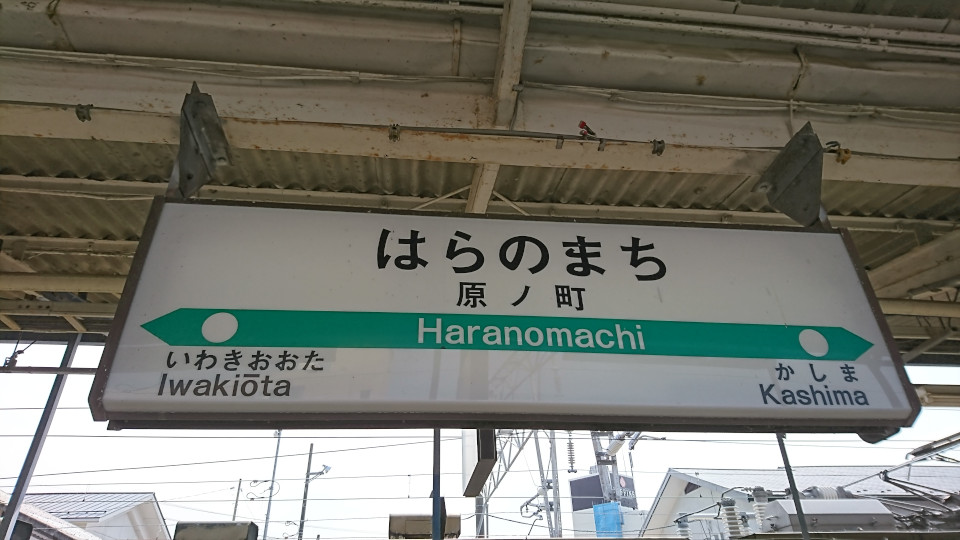
\includegraphics[width=0.7\linewidth]{haranomachi.jpg}
  \end{center}

  \footnotesize
  ここ数か月よく行っているんですが\\
  原ノ味フォントとは関係ありません。。。
\end{frame}

% Insert limited introduction here

\section*{目次}
\begin{frame}\frametitle{}\tiny\setlength{\columnseprule}{1pt}
  \begin{multicols}{2}%
    \tableofcontents
  \end{multicols}
\end{frame}

\section{はじめに}
\begin{frame}\frametitle{}
  \centering
  \usebeamerfont{frametitle}\usebeamercolor[fg]{frametitle}はじめに
\end{frame}

\begin{frame}\frametitle{はじめに}
  \begin{itemize}
  \item 源ノフォント
    \begin{itemize}
    \item 源ノ明朝・源ノ角ゴシック
    \item オープンソースのPan-CJKフォント
    \item 明朝・ゴシックそれぞれ7ウェイト
    \item CID-keyed OpenType/CFFフォント
    \end{itemize}

    \pause
  \item 日本語OpenType/CFFフォントとの違い
    \begin{itemize}
    \item 従来はAdobe-Japan1 (AJ1)
    \item 源ノフォントはAdobe-Identity-0 (AI0)
    \end{itemize}
  \end{itemize}
\end{frame}

\begin{frame}\frametitle{\TeX で源ノフォント}
  \begin{itemize}
  \item 最新の\TeX \ Live 2019では使用可能
    \begin{itemize}
    \item 関係各位のご尽力で\\
      AI0対応、源ノフォント対応が進んだ
    \end{itemize}
    
    \pause
  \item ただし、一部で使用困難や問題発生
    \begin{itemize}
    \item AI0なので…AJ1ではないので…
    \end{itemize}
  \end{itemize}
\end{frame}

\begin{frame}\frametitle{原ノ味フォント}
  \begin{itemize}
  \item 源ノフォントをAJ1へ組み替え
    \begin{itemize}
    \item AI0に起因する問題を解決
      \begin{itemize}
      \item 各種\TeX エンジン
      \item DVIドライバ
      \item Ghostscript
      \end{itemize}
    \end{itemize}

    \pause
  \item AJ1とAI0は何が違うのか?
  \item AI0だとどんな問題があるのか?
  \end{itemize}
\end{frame}

\section{AJ1とAI0}
\begin{frame}\frametitle{}
  \centering
  \usebeamerfont{frametitle}\usebeamercolor[fg]{frametitle}AJ1とAI0
\end{frame}

\subsection{フォントとCID}
\begin{frame}\frametitle{フォント}
  \begin{itemize}
  \item \textbf{いくつの文字}について\\
    \textbf{統一されたデザイン}の\\
    \textbf{グリフ}(字形)\\
    を収録したもの
  \item 様々な形式がある
    \begin{itemize}
    \item OpenTypeもその一つ
    \end{itemize}
  \end{itemize}
\end{frame}

\begin{frame}\frametitle{源ノフォント}
  \begin{itemize}
  \item いくつかの文字
    \begin{itemize}
    \item Pan-CJKフォント
      \begin{itemize}
      \item CJK各言語の多数の文字を収録
      \end{itemize}
    \end{itemize}
  \item 統一されたデザイン
    \begin{itemize}
    \item 同じフォント内の文字は\\
      デザインが統一されている
      \begin{itemize}
        \item 明朝体・ゴシック体、ウェイトなど
      \end{itemize}
    \end{itemize}
  \item グリフ(字形)
    \begin{itemize}
    \item 収録した文字のアウトラインデータ\\
      を持っている
    \end{itemize}
  \item 形式
    \begin{itemize}
    \item CID-keyed OpenType/CFF
    \end{itemize}
  \end{itemize}
\end{frame}

\begin{frame}\frametitle{CID (Character ID)}
  \begin{itemize}
  \item 様々な種類の文字(Character)\\
    ひとつひとつに付けられた\\
    ユニークな識別子(ID)
  \item 0から始まる番号
    \begin{itemize}
    \item 0番はCID+0、1番はCID+1のように表記
    \end{itemize}
  \end{itemize}
\end{frame}

\begin{frame}\frametitle{CID-keyed}
  \begin{itemize}
  \item CIDキー方式
    \begin{itemize}
    \item CIDをキーとして\\
      使いたい文字のグリフを指定する方式
    \end{itemize}
  \item アプリケーションの動作
    \begin{itemize}
    \item 使いたい文字をCID番号で指定
    \item そのグリフのアウトラインを取得
    \item 表示や印字をする
    \end{itemize}
  \end{itemize}

  \begin{center}
    \footnotesize
    \begin{tabular}{c|c}
      使いたい文字 & CID(AJ1フォントの場合) \\
      \hline
      あ & CID+843 \\
      漢 & CID+1533 \\
      ☃ & CID+8218
    \end{tabular} \\
    使いたい文字とCIDの例
  \end{center}
\end{frame}

\begin{frame}\frametitle{文字コード}
  \begin{itemize}
  \item 普通のアプリはCIDを知らない
    \begin{itemize}
    \item \textbf{文字コード}を\textbf{符号化}(エンコーディング)\\
      したもので取り扱っている
    \end{itemize}
  \item 文字コード
    \begin{itemize}
    \item JIS X 0208、Unicodeなど
    \end{itemize}
  \end{itemize}
\end{frame}
      
\begin{frame}\frametitle{文字コード規格の例}
  \begin{itemize}
    \item JIS X 0208
      \begin{itemize}
      \item 日本語でよく使われる文字を集め、\\
        それらを識別する番号を付与したもの
        \begin{itemize}
        \item 区と点それぞれ10進数や、\\
          2桁の10進数2つをハイフンでつなぐ\\
          などで表記する
        \end{itemize}
      \item 符号化
        \begin{itemize}
        \item ISO-2022-JP(JISコード)・Shift\_JIS・EUC-JPなど
        \end{itemize}
      \end{itemize}
  \end{itemize}

  \begin{center}
    \footnotesize
    \begin{tabular}{c|cc|c|c|c}
      & \multicolumn{5}{c}{JIS X 0208} \\
      \cline{4-6}
      文字 & & & ISO-2022-JP & Shift\_JIS & EUC-JP \\
      \hline
      あ & \multicolumn{1}{c @{/}}{4区2点} & 04-02
      & \texttt{24 22} & \texttt{82 A0} & \texttt{A4 A2} \\
      漢 & \multicolumn{1}{c @{/}}{20区33点} & 20-33
      & \texttt{34 41} & \texttt{8A BF} & \texttt{B4 C1}
    \end{tabular} \\
    文字と符号化の例
  \end{center}
\end{frame}

\begin{frame}\frametitle{文字コード規格の例}
  \begin{itemize}
  \item Unicode
    \begin{itemize}
    \item JIS X 0208も含めた世界中の\\
      様々な規格にある文字などを集め、\\
      それらを識別する番号を付与したもの
      \begin{itemize}
      \item ``U+''の後に16進数4~6桁を付け表記
      \end{itemize}
    \item 符号化
      \begin{itemize}
        \item UTF-8・UTF-16・UTF-32など
      \end{itemize}
    \end{itemize}
  \end{itemize}

  \begin{center}
    \footnotesize
    \begin{tabular}{c|c|c|c|c}
      & \multicolumn{4}{c}{Unicode} \\
      \cline{3-5}
      文字 & & UTF-8 & UTF-16 & UTF-32 \\
      \hline
      あ & U+3042 & \texttt{E3 81 82} & \texttt{3042} & \texttt{00003042} \\
      漢 & U+6F22 & \texttt{E6 BC A2} & \texttt{6F22} & \texttt{00006F22} \\
      ☃ & U+2603 & \texttt{E2 98 83} & \texttt{2603} & \texttt{00002603}
    \end{tabular} \\
    文字と符号化の例
  \end{center}
\end{frame}

\begin{frame}\frametitle{文字コードとCID}
  \begin{itemize}
  \item 全く異なった体系にある
  \item 変換テーブル(マッピング)を用意して\\
    CIDに変換する必要がある
  \item CIDを使ってグリフを指定し \\
    アウトラインを取得する
  \end{itemize}

  \begin{center}
    \footnotesize
    \input{conv_to_cid.pdf_tex}
  \end{center}
\end{frame}

\begin{frame}\frametitle{文字コレクション}
  \begin{itemize}
  \item CID-keyedフォントが持つ情報
    \begin{itemize}
    \item どのような文字を収録しているかを示す
    \end{itemize}
  \item ROSとも呼ばれる
    \begin{itemize}
    \item ``Registry''(登録者)
    \item ``Ordering''(版)
    \item ``Supplement''(追補)
    \end{itemize}
    \item これらをハイフンでつないで呼ばれる
  \end{itemize}

  \begin{center}
    \footnotesize
    \begin{tabular}{c|c@{-}c@{-}c}
      & Registry & Ordering & Supplement \\
      \hline
      AJ1-7 & Adobe & Japan1 & 7 \\
      AI0   & Adobe & Identity & 0
    \end{tabular} \\
    文字コレクションの例
  \end{center}
\end{frame}

\subsection{Adobe-Japan1 (AJ1)}
\begin{frame}\frametitle{Adobe-Japan1 (AJ1)}
  \begin{itemize}
  \item 日本語で使われる様々な文字を集め、 \\
    識別のためCIDを割り当てたもの
  \item 最初のAdobe-Japan1-0 (AJ1-0)から \\
    最新のAdobe-Japan1-7 (AJ1-7)まである
  \end{itemize}

  \begin{center}
    \scriptsize
  \begin{tabular}{l|r|rcr|r|r}
    & \multicolumn{1}{c|}{制定年}
    & \multicolumn{3}{c|}{追加されたCID}
    & \multicolumn{1}{c|}{追加数}
    & \multicolumn{1}{c}{合計} \\
    \hline
    AJ1-0 & 1992 &     0 & ~ &  8283 & 8,284 &  8,284 \\
    AJ1-1 & 1993 &  8284 & ~ &  8358 &    75 &  8,359 \\
    AJ1-2 & 1993 &  8359 & ~ &  8719 &   361 &  8,720 \\
    AJ1-3 & 1998 &  8720 & ~ &  9353 &   634 &  9,354 \\
    AJ1-4 & 2000 &  9354 & ~ & 15443 & 6,090 & 15,444 \\
    AJ1-5 & 2002 & 15444 & ~ & 20316 & 4,873 & 20,317 \\
    AJ1-6 & 2004 & 20317 & ~ & 23057 & 2,741 & 23,058 \\
    AJ1-7 & 2019 & 23058 & ~ & 23059 &     2 & 23,060
  \end{tabular}
  \end{center}
\end{frame}

\begin{frame}\frametitle{AJ1の例}
  \begin{center}
    \footnotesize
  \begin{tabular}{c|c|c}
         & Unicode & AJ1 \\
    \hline
    あ   & U+3042  & CID+843 \\
    漢   & U+6F22  & CID+1533 \\
    ☃   & U+2603  & CID+8218 \\
    \arrayrulecolor[gray]{0.7}\hline\arrayrulecolor[gray]{0}
    {\gtfamily \CID{23058}} & U+32FF & CID+23058 \\
    {\gtfamily \CID{23059}} & 〃     & CID+23059 \\
    \arrayrulecolor[gray]{0.7}\hline\arrayrulecolor[gray]{0}
    \CID{7634} & U+98F4  & CID+7634 \\
    \CID{1151} & 〃      & CID+1151 \\
    \arrayrulecolor[gray]{0.7}\hline\arrayrulecolor[gray]{0}
    \CID{1887} & U+898B  & CID+1887 \\
    \CID{1887} & U+2F92  & 〃
  \end{tabular} \\
  文字とUnicode、AJ1 CIDの例
  \end{center}
\end{frame}

\begin{frame}\frametitle{見た目が異なれば別のCID}
  \begin{itemize}
  \item 横書き用と縦書き用
    \begin{itemize}
    \item Unicodeは区別しない
    \end{itemize}
  \end{itemize}

  \begin{center}
    \footnotesize
  \begin{tabular}{c|c|c|c}
         & 縦横 & Unicode & AJ1 \\
    \hline
    {\gtfamily \CID{23058}} & 横書き & U+32FF & CID+23058 \\
    {\gtfamily \CID{23059}} & 縦書き & 〃     & CID+23059 \\
  \end{tabular}
  \end{center}

  \begin{itemize}
  \item JIS2004字形とJIS90字形
    \begin{itemize}
    \item Unicodeは区別しない
    \end{itemize}
  \end{itemize}

  \begin{center}
    \footnotesize
  \begin{tabular}{c|c|c|c}
         & 字形 & Unicode & AJ1 \\
    \hline
    \CID{7634} & JIS2004 & U+98F4  & CID+7634 \\
    \CID{1151} & JIS90   & 〃      & CID+1151 \\
  \end{tabular}
  \end{center}
\end{frame}

\begin{frame}\frametitle{見た目が同じなら同じCID}
  \begin{itemize}
  \item 普通の漢字と部首
    \begin{itemize}
    \item Unicodeは区別する
    \end{itemize}
  \end{itemize}

  \begin{center}
    \footnotesize
  \begin{tabular}{c|c|c|c}
         & 由来 & Unicode & AJ1 \\
    \hline
    \CID{1887} & 漢字 & U+898B  & CID+1887 \\
    \CID{1887} & 部首 & U+2F92  & 〃
  \end{tabular}
  \end{center}
\end{frame}

\begin{frame}\frametitle{変換テーブル(マッピング)}
  \begin{itemize}
  \item 文字コードからCIDに変換する方法は \\
    2種類ある
    \begin{itemize}
    \item CMapリソース
      \begin{itemize}
      \item \pTeX /\upTeX \ + dvipdfmx/dvipsなどで使用 \\
        (AJ1フォントの場合)
      \item フォントファイルとは別のファイルを指定
      \end{itemize}
    \item cmapテーブル
      \begin{itemize}
      \item \LuaTeX /\XeTeX などで使用
      \item フォントファイルに内蔵されている
      \end{itemize}
    \end{itemize}
  \end{itemize}
\end{frame}

\begin{frame}\frametitle{CMapリソース}
  \begin{itemize}
  \item 入出力の種類別にファイルがある
  \end{itemize}

  \begin{center}
    \footnotesize
    \begin{tabular}{l|c|c|c}
      & 入力 & \multicolumn{2}{c}{出力(AJ1)} \\
      \cline{3-4}
      &      & 字形 & 縦横 \\
      \hline
      \texttt{H}                  & ISO-2022-JP (JIS) & JIS90   & 横書き \\
      \texttt{V}                  & ISO-2022-JP (JIS) & JIS90   & 縦書き \\
      \texttt{2004-H}             & ISO-2022-JP (JIS) & JIS2004 & 横書き \\
      \texttt{2004-V}             & ISO-2022-JP (JIS) & JIS2004 & 縦書き \\
      \texttt{UniJIS-UTF16-H}     & UTF-16            & JIS90   & 横書き \\
      \texttt{UniJIS-UTF16-V}     & UTF-16            & JIS90   & 縦書き \\
      \texttt{UniJIS2004-UTF16-H} & UTF-16            & JIS2004 & 横書き \\
      \texttt{UniJIS2004-UTF16-V} & UTF-16            & JIS2004 & 縦書き
    \end{tabular} \\
    CMapリソースの例
  \end{center}
\end{frame}

\begin{frame}\frametitle{\pTeX}
  \begin{itemize}
  \item DVIファイルはJISコード
  \item dvipdfmxマップファイルの設定
    \begin{itemize}
    \item JISコード用CMapを \\
      使用する字形・縦横別に指定する
      \begin{itemize}
        \item \texttt{H}, \texttt{V}, \texttt{2004-H}, \texttt{2004-V}
      \end{itemize}
    \end{itemize}
  \item dvipdfmxの動作
    \begin{centering}
      \footnotesize
      \input{ptex_to_cid.pdf_tex}
    \end{centering}
  \end{itemize}
\end{frame}

\begin{frame}\frametitle{cmapテーブル}
  \begin{itemize}
  \item OpenTypeに内蔵されている
  \item 基本的に1種類しかない
    \begin{itemize}
    \item 入力:Unicodeのみ
    \item 出力:字形固定、横書きのみ
    \end{itemize}
  \item OpenType featureで \\
    字形や縦書きを切り替える
    \begin{itemize}
    \item GSUBテーブル
    \end{itemize}
  \end{itemize}
\end{frame}

\begin{frame}\frametitle{\LuaTeX}
  \begin{itemize}
  \item \TeX ファイルはUnicode (UTF-8)
  \item フォントの指定のみ
    \begin{itemize}
    \item マッピングの指定は無し
    \item 必要に応じてOpenType featureの指定
    \end{itemize}
  \item \LuaTeX の動作
    \begin{centering}
      \footnotesize
      \input{luatex_to_cid.pdf_tex}
    \end{centering}
  \end{itemize}
\end{frame}

\subsection{Adobe-Identity-0 (AI0)}
\begin{frame}\frametitle{Adobe-Identity-0 (AI0)}
  \begin{itemize}
  \item AJ1
    \begin{itemize}
    \item 「日本語のため」の文字コレクション
    \item 以下は収録できない
      \begin{itemize}
      \item AJ1で定義されていない文字\\
        (日本語で使われない)
      \item 同じ文字の複数バリエーション
      \end{itemize}
    \item フォントが違っても同じCIDは同じ文字
    \end{itemize}
  \item AI0
    \begin{itemize}
    \item 「特別な目的」の文字コレクション
      \begin{itemize}
      \item 何も事前に定義されていない
      \item フォント制作者が自分で自由に決める
      \end{itemize}
    \item フォントが違えば同じCIDでも違う文字
    \end{itemize}
  \end{itemize}
\end{frame}

\begin{frame}\frametitle{源ノフォント}
  \begin{itemize}
  \item 明朝とゴシック間でCIDが異なる
  \item バージョン間でCIDが異なる
  \end{itemize}

  \begin{center}
    \tiny
  \begin{tabular}{c|c|c|c|c}
         &         &          & \multicolumn{2}{c}{AI0} \\
    \cline{4-5}
         & Unicode & AJ1      & 源ノ明朝 & 源ノ角ゴシック \\
         &         &          & 1.001    & 2.001 \\
    \hline
    あ   & U+3042  & CID+843  & CID+1461 & CID+1461 \\
    漢   & U+6F22  & CID+1533 & CID+24743 & CID+24227 \\
    ☃   & U+2603  & CID+8218 & CID+1274 & CID+1281 \\
    \arrayrulecolor[gray]{0.7}\hline\arrayrulecolor[gray]{0}
    {\gtfamily \CID{23058}} & U+32FF & CID+23058 & --- & CID+2184 \\
    {\gtfamily \CID{23059}} & 〃     & CID+23059 & --- & CID+65359 \\
    \arrayrulecolor[gray]{0.7}\hline\arrayrulecolor[gray]{0}
    \CID{7634} & U+98F4  & CID+7634 & CID+45263 & CID+44358 \\
    \CID{1151} & 〃      & CID+1151 & CID+61214 & CID+62049 \\
    \arrayrulecolor[gray]{0.7}\hline\arrayrulecolor[gray]{0}
    \CID{1887} & U+898B  & CID+1887 & CID+38198 & CID+37348 \\
    \CID{1887} & U+2F92  & 〃       & 〃        & 〃
  \end{tabular}
  \end{center}
\end{frame}

\begin{frame}\frametitle{CMapリソース}
  \begin{itemize}
  \item 源ノフォント用は一応存在する
    \begin{itemize}
    \item 入力:UTF-16, UTF-32のみ
      \begin{itemize}
      \item DVIファイルがJISコードの\pTeX で使えない
      \end{itemize}
    \item 出力:JIS2004字形、横書きのみ
      \begin{itemize}
        \item 字形切り替え、縦書きができない
      \end{itemize}
    \end{itemize}
  \item インストール・設定が煩雑
    \begin{itemize}
    \item 明朝・ゴシックで別ファイルになっている
    \item バージョンアップすると \\
      CMapリソースも入れ替える必要あり
    \end{itemize}
  \item 事実上「使えない」
  \end{itemize}
\end{frame}

\begin{frame}\frametitle{cmapテーブル}
  \begin{itemize}
  \item AI0でもAJ1と同様に使える
    \begin{itemize}
    \item \LuaTeX /\XeTeX
      \begin{itemize}
      \item 字形切替や縦書きもAJ1と同程度に利用可
      \item 設定でAJ1/AI0を意識する必要なし \\
        (cmapテーブルはフォントファイルに内蔵)
      \end{itemize}
    \end{itemize}
  \item \upTeX \ + dvipdfmxなら利用可能
    \begin{itemize}
    \item マップファイルで設定可
    \item ただし制約あり
      \begin{itemize}
      \item OTFパッケージは大部分が利用不可
      \item AJ1と文字幅が異なると問題が発生、など
      \end{itemize}
    \end{itemize}
  \end{itemize}
\end{frame}

\section{源ノフォントを使う}
\begin{frame}\frametitle{}
  \centering
  \usebeamerfont{frametitle}\usebeamercolor[fg]{frametitle}源ノフォントを使う
\end{frame}

\begin{frame}\frametitle{それでも源ノフォントを使う}
  \begin{itemize}
  \item AI0の問題を回避して使う方法を考える
  \item ただし、いずれの方法も
    \begin{itemize}
    \item 設定が煩雑
    \item 制約がある
    \end{itemize}
  \item 注意が必要
  \end{itemize}
\end{frame}

\subsection{\pTeX で使う}
\begin{frame}\frametitle{\pTeX で使うには}
  \begin{itemize}
  \item 使う方法は(一応)ある
    \begin{itemize}
    \item CMapリソースを作成する
    \item VFを使う
    \item DVIファイルを書き換える
    \end{itemize}
  \end{itemize}
\end{frame}

\subsection{\upTeX で使う}
\begin{frame}\frametitle{\upTeX で使うには}
  \begin{itemize}
  \item dvipdfmxなら使える
  \item dvipsでは…
    \begin{itemize}
    \item 源ノフォントのCMapリソースを使う
    \end{itemize}
  \end{itemize}
\end{frame}

\subsection{\TeX エンジンを移行する}
\begin{frame}\frametitle{\TeX エンジンを移行する}
  \begin{itemize}
  \item \pLaTeX 専用のクラスファイルを \\
    何とかする
    \begin{itemize}
    \item 新規作成する
    \item 改変する
    \end{itemize}
  \end{itemize}
\end{frame}

\section{原ノ味フォント}
\begin{frame}\frametitle{}
  \centering
  \usebeamerfont{frametitle}\usebeamercolor[fg]{frametitle}原ノ味フォント
\end{frame}

\begin{frame}\frametitle{源ノフォントの問題}
  \begin{itemize}
  \item 一部の環境
    \begin{itemize}
    \item \pTeX
    \item \upTeX \ + dvips
    \item OTFパッケージ、など
    \end{itemize}
  \item 利用困難
    \begin{itemize}
    \item 設定が煩雑
    \item 制約がある、など
    \end{itemize}
  \end{itemize}
\end{frame}

\begin{frame}\frametitle{原ノ味フォント}
  \begin{itemize}
  \item 源ノフォントの問題はAI0が原因
    \begin{itemize}
    \item AJ1なら発生しない…
    \end{itemize}
  \item AJ1へ組み替えればいいのでは?
  \item そこで\alert{原ノ味フォント}を制作
  \end{itemize}
\end{frame}

\begin{frame}\frametitle{原ノ味フォントとは}
  \begin{itemize}
  \item 「原ノ味」の意味
    \begin{itemize}
    \item 源ノフォントから「\ltjruby{氵}{さんずい}」を取った
      \begin{itemize}
      \item グリフやテーブルが抜けているので
      \end{itemize}
    \item AJ1をもじる
      \begin{itemize}
      \item AJIにして音から「味」をあてた
      \end{itemize}
    \item 「ノ」はカタカナ
    \end{itemize}
  \item オープンソース
    \begin{itemize}
    \item SIL Open Font License
      \begin{itemize}
      \item 源ノフォントの派生フォントなので
      \end{itemize}
    \end{itemize}
  \end{itemize}
\end{frame}

\subsection{制作の経緯}
\begin{frame}\frametitle{制作の経緯}
  \begin{itemize}
  \item \texttt{ipsj.cls}で源ノフォントを \\
    使いたい
    \begin{itemize}
    \item 情報処理学会\LaTeX スタイルファイル
    \item \pLaTeX 専用
    \end{itemize}
  \item しかし、様々な問題が発生、 \\
    一筋縄ではいかない
  \end{itemize}
\end{frame}

\begin{frame}\frametitle{制作の経緯}
  \begin{itemize}
  \item 源ノフォントはオープンソース
    \begin{itemize}
    \item 一定の条件下で改変や \\
      再配布が認められている
    \end{itemize}
  \item 源ノフォントのグリフを使った \\
    AJ1フォントが作れるのでは?
  \item ということで制作を開始
  \end{itemize}
\end{frame}

\subsection{搭載グリフ}
\begin{frame}\frametitle{搭載グリフ}
  \begin{itemize}
  \item 漢字
    \begin{itemize}
    \item AJ1-6漢字グリフすべて搭載
      \begin{itemize}
      \item ルビ用の「注」は非搭載 \\
        (AJ1漢字グリフ範囲外)
      \end{itemize}
    \item JIS X 0208漢字グリフすべて搭載
    \item JIS X 0213漢字グリフすべて搭載
    \end{itemize}
  \end{itemize}
\end{frame}

\begin{frame}\frametitle{搭載グリフ}
  \begin{itemize}
  \item 非漢字 \\
    (ひらがな、カタカナ、英数字、記号類)
    \begin{itemize}
    \item JIS X 0208横書きグリフすべて搭載
    \item JIS X 0208縦書きグリフは \\
      以下4グリフを除きすべて搭載
      \begin{itemize}
      \item 「‖」「\ltjjachar`°」「\ltjjachar`′」「\ltjjachar`″」
      \end{itemize}
    \end{itemize}
  \item JIS X 0213非漢字グリフには抜けあり
  \item その他AJ1-6非漢字グリフには抜けあり
  \end{itemize}
\end{frame}

\begin{frame}\frametitle{文字幅}
  \begin{itemize}
  \item 非漢字の一部に文字幅を強制的に \\
    AJ1へ合わせたものがある
    \begin{itemize}
    \item ギリシャ文字、キリル文字、一部の記号類
    \end{itemize}
  \item 不格好な表示になることがある
    \begin{itemize}
    \item 文字幅は正しいので \\
      後続文字の位置がズレるような \\
      問題は発生しない
    \end{itemize}
  \end{itemize}
\end{frame}

\subsection{生成プログラム}
\begin{frame}\frametitle{生成プログラム}
  \begin{itemize}
  \item オープンソースで公開している
    \begin{itemize}
      \item 自分で原ノ味フォントを生成できる
      \item カスタマイズも可能
    \end{itemize}
  \end{itemize}
\end{frame}

\begin{frame}\frametitle{動作}
  \begin{itemize}
  \item 源ノフォントのOTFファイルを \\
    fonttoolsのttxでXMLにする
  \item このXMLやCMapリソースなどから \\
    CIDの対照表を作る
  \item 対照表に基づいてXMLのCIDを変換
  \item 最後に再びttxでOTFファイルを生成
  \end{itemize}
\end{frame}

\begin{frame}\frametitle{CIDの対応}
  \begin{itemize}
  \item 源ノフォントはAI0フォント
    \begin{itemize}
    \item CIDの並び方がAJ1とは異なる
    \end{itemize}
  \item AJ1化するには \\
    AI0 CID→AJ1 CID \\
    対照表が必要
  \item 自動で対照表を作成する
    \begin{itemize}
    \item グリフ数が多く人手では困難
      \begin{itemize}
        \item 日本語用でも2万近い数
      \end{itemize}
    \end{itemize}
  \end{itemize}
\end{frame}

\subsection{\pTeX ・\upTeX で使う}
\begin{frame}\frametitle{\pTeX ・\upTeX で使う}
  \begin{itemize}
  \item 源ノフォントと異なり簡単に使える
    \begin{itemize}
    \item フォントファイルとマップファイルを \\
      適切に配置
      \begin{itemize}
      \item マップファイルも \\
        原ノ味フォントのサイトで配布している
      \end{itemize}
    \item \texttt{kanji-config-updmap}コマンドで設定
    \end{itemize}
  \end{itemize}
\end{frame}

\begin{frame}\frametitle{\pTeX ・\upTeX で使う}
  \begin{itemize}
  \item 注意点
    \begin{itemize}
    \item 非搭載グリフは使えない
      \begin{itemize}
      \item □に\ltjjachar`×を重ねたようなダミーグリフが出る
      \end{itemize}
    \item 文字幅の問題で一部に表示が \\
      不格好なグリフがある
      \begin{itemize}
      \item 源ノフォントのような \\
        後続文字の位置がズレる問題は無し
      \end{itemize}
    \end{itemize}
  \end{itemize}
\end{frame}

\subsection{その他の環境で使う}
\begin{frame}\frametitle{その他の環境で使う}
  \begin{itemize}
  \item \LuaTeX 、\XeTeX 、LilyPond
    \begin{itemize}
    \item 他のフォントと同様に利用可能
    \item IVSやOpenType featureも使える
    \end{itemize}
  \end{itemize}
\end{frame}

\section{ToUnicode CMap}
\begin{frame}\frametitle{}
  \centering
  \usebeamerfont{frametitle}\usebeamercolor[fg]{frametitle}ToUnicode CMap
\end{frame}

\begin{frame}\frametitle{ToUnicode CMap}
  \begin{itemize}
  \item PDF中の文字がCIDで指定
    \begin{itemize}
    \item Unicodeなどは失われている
    \end{itemize}
  \item テキスト抽出には \\
    CID→Unicode \\
    というテーブルが必要
  \item これがToUnicode CMap
  \end{itemize}
\end{frame}

\begin{frame}\frametitle{テキスト抽出}
  \begin{itemize}
  \item PDFからテキスト抽出
    \begin{itemize}
    \item PDF viewrからのコピー&ペーストなど
    \end{itemize}
  \item AJ1フォント
    \begin{itemize}
    \item PDFにToUnicode CMapが無くてもOK
    \item PDF viewerが持っていればよい
    \end{itemize}
  \item AI0フォント
    \begin{itemize}
    \item PDFにToUnicode CMapが必要
    \end{itemize}
  \end{itemize}
\end{frame}

\subsection{ToUnicode CMapの自動生成}
\begin{frame}\frametitle{ToUnicode CMapの自動生成}
  \begin{itemize}
  \item dvipdfmx (\pTeX /\upTeX ) \\
    xdvipdfmx (\XeTeX )
    \begin{itemize}
    \item AJ1フォント:自動生成・埋め込みせず
    \item AI0フォント:自動生成・埋め込みする
    \end{itemize}
  \item \LuaTeX
    \begin{itemize}
    \item 全フォント:自動生成・埋め込みする
    \end{itemize}
  \end{itemize}
\end{frame}

\begin{frame}\frametitle{逆変換による自動生成}
  \begin{itemize}
  \item 生成方法
    \begin{itemize}
    \item PDFで使用するCIDで \\
      cmapテーブルを参照
    \item この逆変換でToUnicode CMapを生成
    \end{itemize}
  \end{itemize}
\end{frame}

\begin{frame}\frametitle{逆変換による自動生成}
  \begin{itemize}
  \item 問題1(いわゆる部首問題)
    \begin{itemize}
    \item CID+1887はU+898B?それともU+2F92?
    \end{itemize}
  \end{itemize}

  \begin{center}
    \footnotesize
  \begin{tabular}{c|c|c|c}
         & 由来 & Unicode & AJ1 \\
    \hline
    \CID{1887} & 漢字 & U+898B  & CID+1887 \\
    \CID{1887} & 部首 & U+2F92  & 〃
  \end{tabular}
  \end{center}

  \begin{itemize}
  \item どちらがよりふさわしいか
    \begin{itemize}
    \item 個々のCIDによって異なる
    \item 現状は「部首」のブロックを決めて \\
      選択されないようにして回避している
    \end{itemize}
  \end{itemize}
\end{frame}

\begin{frame}\frametitle{逆変換による自動生成}
  \begin{itemize}
  \item 問題2(非デフォルトCIDが抜ける)
    \begin{itemize}
    \item CID+23059(縦書き)
    \item CID+1151(JIS90字形)
      \begin{itemize}
      \item JIS2004フォントの場合
      \end{itemize}
    \end{itemize}
  \end{itemize}

  \begin{center}
    \footnotesize
  \begin{tabular}{c|c|c|cc}
         & 種類 & Unicode & AJ1 \\
    \cline{1-4}
    {\gtfamily \CID{23058}} & 横書き & U+32FF & CID+23058 & ←〇 \\
    {\gtfamily \CID{23059}} & 縦書き & 〃     & CID+23059 & ←\ltjjachar`× \\
    \CID{7634} & JIS2004字形 & U+98F4  & CID+7634 & ←〇 \\
    \CID{1151} & JIS90字形   & 〃      & CID+1151 & ←\ltjjachar`×
  \end{tabular}
  \end{center}

  \begin{itemize}
  \item cmapテーブルに載っていない \\
    →逆変換不可→テキスト抽出できない
  \end{itemize}
\end{frame}

\begin{frame}\frametitle{逆変換による自動生成}
  \begin{itemize}
  \item 問題3(非デフォルトCIDが化ける)
    \begin{itemize}
    \item cmapテーブル
      \begin{itemize}
      \item 開き括弧「(」U+FF08→CID+674
      \end{itemize}
    \item GSUBテーブルvert(縦書き)
      \begin{itemize}
      \item CID+674→CID+7899「︵」
      \end{itemize}
    \item 逆変換生成したToUnicode CMap
      \begin{itemize}
      \item CID+7899→U+FE35
      \end{itemize}
    \end{itemize}
  \item 本来U+FF08が抽出されるべきだが \\
    U+FE35になる
  \end{itemize}
\end{frame}

\subsection{調整済のToUnicode CMap}
\begin{frame}\frametitle{調整済のToUnicode CMap}
  \begin{itemize}
  \item 調整済のAJ1用ToUnicode CMapがある
    \begin{itemize}
    \item 問題1~3が起きにくいよう \\
      配慮されている
    \end{itemize}
  \item PDF viewrがこれを持っている
    \begin{itemize}
    \item AJ1ならPDFにToUnicode CMapが \\
      埋め込まれてなくてもテキスト抽出できる
    \item PDFのファイルサイズが小さくて済む
    \item 問題1~3が起きにくい
    \end{itemize}
  \end{itemize}
\end{frame}

\subsection{PDF/A-2u}
\begin{frame}\frametitle{PDF/A-2u}
  \begin{itemize}
  \item PDF/A
    \begin{itemize}
    \item 遠い将来のPDF viewerでも \\
      利用できるよう配慮したPDFの規格
    \item 通常のPDF規格をベースに \\
      守るべき事項が追加されている
    \end{itemize}
  \item PDF/A-2u
    \begin{itemize}
    \item PDF/Aの一つ
    \item テキスト抽出(Unicode取得)できる \\
      ことが必須
    \end{itemize}
  \end{itemize}
\end{frame}

\begin{frame}\frametitle{PDF/A-2u}
  \begin{itemize}
  \item PDF/A作成
    \begin{itemize}
    \item 本件公開アブストラクトのPDFがPDF/A-2u準拠
      \begin{itemize}
      \item ※現在TeXConf 2019公式ページ \\
        にあるPDFは非準拠
      \end{itemize}
    \item GitHubにて\TeX ソース公開中
    \end{itemize}
  \item バリデーション
    \begin{itemize}
    \item veraPDFでバリデーションチェック可能
    \item 公開アブストラクトPDF(GitHub版) \\
      はveraPDF 1.15.8で準拠の確認済
    \end{itemize}
  \end{itemize}
\end{frame}

\begin{frame}\frametitle{テキスト抽出の条件}
  \begin{itemize}
  \item veraPDFドキュメントより
    \begin{itemize}
    \item 基本的にはToUnicode CMapが必要
    \item 例外的に無くてもよい条件がある
    \item そのうちの一つがAJ1の場合
    \end{itemize}
  \item AJ1ならPDFにToUnicode CMapが \\
    \alert{無くてもよい}
    \begin{itemize}
    \item 無くてもPDF/A-2u準拠できる \\
      →テキスト抽出できる
    \end{itemize}
  \item AI0にはないメリット
  \end{itemize}
\end{frame}

\section{\LuaTeX とToUnicode CMap}
\begin{frame}\frametitle{}
  \centering
  \usebeamerfont{frametitle}%
  \usebeamercolor[fg]{frametitle}\LuaTeX とToUnicode CMap
\end{frame}

\begin{frame}\frametitle{\LuaTeX とToUnicode CMap}
  \begin{itemize}
  \item dvipdfmx/xdvipdfmx
    \begin{itemize}
    \item AJ1フォントならToUnicode CMapを \\
      生成せず、埋め込まない
    \end{itemize}
  \item \LuaTeX
    \begin{itemize}
    \item AJ1フォントでもToUnicode CMapを \\
      生成して、埋め込む
    \item ROSをAI0へ書き換えてしまう
    \item つまり、AJ1フォントでも \\
      逆変換問題が発生してしまう
    \end{itemize}
  \end{itemize}
\end{frame}

\subsection{ToUnicode CMap削除}
\begin{frame}\frametitle{ToUnicode CMap削除}
  \begin{itemize}
  \item AI0に書き換えてもCIDは変わらない
  \item PDFのROSをAJ1に戻し、 \\
    ToUnicode CMapを削除すると…
  \item 逆変換の問題を解消することができた
    \begin{itemize}
      \item PDFのファイルサイズが小さくなる
      \item 前節の問題1~3が起きにくくなる
      \item AJ1のメリットが得られる
    \end{itemize}
  \end{itemize}
\end{frame}

\subsection{削除ツール}
\begin{frame}\frametitle{削除ツール}
  \begin{itemize}
  \item 自動的にToUnicode CMap削除ができるツールpdf-rm-tucを作成
    \begin{itemize}
      \item \url{https://github.com/trueroad/pdf-rm-tuc}
    \end{itemize}
  \item 公開アブストラクトPDF(GitHub版)は本ツールで削除済
    \begin{itemize}
      \item veraPDF 1.15.8でPDF/A-2u準拠の確認済
    \end{itemize}
  \end{itemize}
\end{frame}

\section{おわりに}
\begin{frame}\frametitle{}
  \centering
  \usebeamerfont{frametitle}\usebeamercolor[fg]{frametitle}おわりに
\end{frame}

\begin{frame}\frametitle{おわりに}
  \begin{itemize}
  \item AJ1とAI0の違い
  \item 源ノフォントと原ノ味フォント
  \item ToUnicode CMapとPDF/A-2u
  \item \LuaTeX 向けToUnicode CMap削除ツール
  \end{itemize}
\end{frame}

\begin{frame}\frametitle{原ノ味フォントの今後}
  \begin{itemize}
  \item 抜けているグリフを埋める?
    \begin{itemize}
    \item 源ノフォントに存在しないグリフ
    \item 使用頻度は低そうだが…
      \begin{itemize}
      \item 和文フォントから使うことは \\
        あまりないのでは???
      \end{itemize}
    \end{itemize}
  \item 埋めるには?
    \begin{itemize}
    \item グリフの「変形」ができるか?
      \begin{itemize}
      \item かなりの実装量が必要
      \end{itemize}
    \item ルビ用などはコピーした方がよいか?
      \begin{itemize}
      \item 全く同じ形状のグリフになるが \\
        ないよりはマシか?
      \end{itemize}
    \end{itemize}
  \end{itemize}
\end{frame}

\begin{frame}\frametitle{その他の話題}
  \begin{itemize}
  \item PDF/Aの解説は少ない?
    \begin{itemize}
    \item 印刷用のPDF/Xはたくさんありそう
    \item 本資料はPDF/A-2u準拠
    \item 本資料が助けになれば幸い
    \end{itemize}
  \item PDF/Aのまま電子署名するツール
    \begin{itemize}
    \item 見つからなかったので実験的に作成 \\
      \url
      {https://gist.github.com/trueroad/0b0a2127aff508caf583265fbef4b644}
    \item クライアント証明書をどうするか
      \begin{itemize}
      \item 有償のものが多い
      \item \href{http://www.cacert.org/}
        {CAcert}は無償だが筆者は保証ポイントが無く
        名前を入れられない
      \end{itemize}
    \end{itemize}
  \end{itemize}
\end{frame}

\begin{frame}\frametitle{関連資料}
  \begin{itemize}
  \item 本資料やアブストラクトについて、 \\
    ソースファイルや関連資料を公開中
    \begin{itemize}
    \item \url{https://github.com/trueroad/tr-TeXConf2019}
    \end{itemize}
  \item 不十分なところや間違いなどあれば \\
    ご連絡ください \\
    正誤表や修正版の公開も検討します
  \end{itemize}
\end{frame}


\end{document}
